\chapter{Resultate und Diskussion}
% =================================================================
\thispagestyle{fancy}
% =================================================================
\section{Eigenfrequenz}
Die verschiedenen Messpunkte wurden gewichtet, um \uline{\textbf{eine}} Zahl mit einer Unsicherheit angeben zu können. Daraus ergab sich für die Eigenfrequenz:
\begin{table}[H]
\centering
\begin{tabular}{l}
$\bar{\omega}=\uuline{(4.8\pm1.1E-04)\;rad/s}$
\end{tabular} 
\end{table}
Für eine graphische Ansicht dieser Resultate dient Abbildung \ref{fig:eigenfrequenz}. Es ist deutlich erkennbar, dass je höher die Startauslenkung gewählt wurde, umso kleiner der Fehler wurde. Bei der Gewichtung wurde deshalb die kleinste Unsicherheit ausschlaggebend, was erklärt, wieso das gewogene Mittel von $\omega$ nahezu gleich dem Wert mit der höchsten Startauslenkung ist.
\section{Amplitudenverlauf}
Im Kapitel \ref{subsec:amplitudenverlauf} in der Abbildung \ref{fig:omega_0} wurden die Daten bereits graphisch Dargstellt. Nach den Berechnungen für $\omega_{0}$, sowie auch deren Unsicherheiten für die vier Runs können als Endresultate festgehalten werden:
\begin{table}[H]
\centering
\begin{tabular}{ll}
\textbf{Run 1}: & $\omega_{0}=\uuline{4.89\pm4.2E-04}\;rad/s$\\
\textbf{Run 2}: & $\omega_{0}=\uuline{4.89\pm1.9E-04}\;rad/s$\\
\textbf{Run 3}: & $\omega_{0}=\uuline{4.91\pm3.0E-04}\;rad/s$\\
\textbf{Run 4}: & $\omega_{0}=\uuline{4.91\pm1.3E-04}\;rad/s$
\end{tabular} 
\end{table}
Bei Betrachtung der Abbildung \ref{fig:omega_0} fällt auf, dass die ersten zwei Runs kleinere Kreisfrequenzen aufweisen. Grund dafür ist die geschwindigkeitsproportionale Reibkraft. Bei den ersten zwei Runs wurden vier Magnete, und bei den zweiten zwei Runs vier Magnete verwendet. Die Unterschiede sind nicht sehr gross, doch sie zeigen auf, dass die Magnete einen Einfluss haben. Bei ganz genauer Betrachtung der vier Messpunkte ist die Kreisfrequenz beim ersten und dritten Run leicht erhöht. Erklärbar ist dies mit der Startauslenkung. Nach Abbildung \ref{fig:messresultate_amplitudenverlauf} waren diese kleiner.
\newpage
\section{Resonanz}
Die beiden Abbildungen \ref{fig:amplitudenresonanz} \& \ref{fig:phasenresonanz} werden nun gegenübergestellt und auf einer Abbildung visualisiert. Um die Verknüpfung der beiden aufzuzeigen wurde der Mittelwert von $\omega_{0}$ mit dessen Fehler berechnet und in der Abbildung \ref{fig:resonanz} graphisch dargestellt. Die in der Fehlerrechnung berechneten Fehler der einzelnen Messpunkten werden hier nicht gezeigt, da diese irrelevant sind und die Quintessenz der Auswertung mittels der Abbildung \ref{fig:resonanz} deutlich genug beschrieben wird.
\begin{figure}[h]
\centering
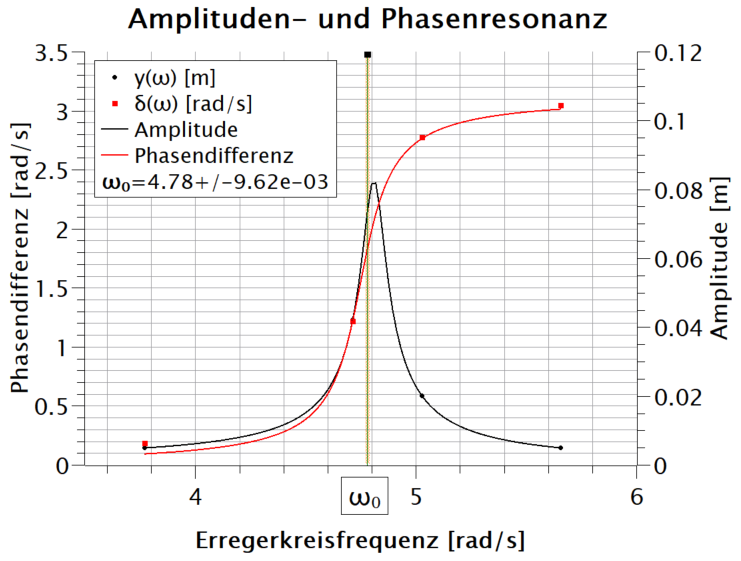
\includegraphics[scale=1.25]{Bilder/resultat_amp_phasresonanz.png} 
\caption{graphische Gegenüberstellung bei der die grüne Linie in der Mitte den Mittelwert von $\omega_{0}$ mit dessen Unsicherheit (orange Fläche) zeigt. Grundsätzlich wird vom Erreger die meiste Energie übertragen, wenn er mit der Eigenfrequenz des Systems schwingt. Dies ist hier gut ersichtlich. Wenn also die Erregerkreisfrequenz bei einer Phasenverschiebung von $\pi/2$ liegt ($\omega=\omega_{0}$), wird die höchste Amplitude (und somit die stärkste Verstärkung der Schwingung) erreicht. Die Werte sind leider etwas ungenau, könnten aber mit mehr Messpunkten verbessert werden.}
\label{fig:resonanz}
\end{figure}






































